\section{Background}
\label{sec:background}

At its foundation, QA utilizes the physical principle of quantum tunneling \cite{ray1989sherrington} to find grounds states for the Ising-Hamiltonian model
\begin{equation}
\mathcal{H}(\text{\boldmath$\sigma$}) = \sum_{i=1}^N h_i\sigma_i + \sum_{i=1}^N \sum_{j=i+1}^N J_{i,j} \sigma_i \sigma_j
\label{eq:hamiltonian}
\end{equation}
where $N$ denotes the number of qubits (quantum bits) involved in the computation (indexed $q_1,\ldots, q_N$), $\sigma_i \in \{-1,1\}$ denotes an eigenstate of $q_i$, $h_i$ denotes the bias of $q_i$, and $J_{i,j}$ denotes the coupler strength between the entangled pair $q_i$ and $q_j$.

Similarly as in AQC, QA achieves the solution to an arbitrary Hamiltonian by beginning from the ground state of an initial Hamiltonian $\mathcal{H}_0$, whose solution is known.
$\mathcal{H}_0$ is then gradually evolved through time into the problem Hamiltonian $\mathcal{H}_1$, via a mathematical homotopy of the form 
\begin{equation}
\mathcal{H}_s(\text{\boldmath$\sigma$}) = (1-s)\mathcal{H}_0(\text{\boldmath$\sigma$}) + s\mathcal{H}_1(\text{\boldmath$\sigma$}).
\label{eq:homotopy}
\end{equation}
Here, the time dependent variable $s$ transitions from $0$ to $1$ during the annealing time \cite{albash2018adiabatic}.

If the transformation (\ref{eq:homotopy}) is adiabatic, meaning that the surrounding temperature is near absolute zero and the rate of change in $\mathcal{H}_s(\text{\boldmath$\sigma$})$ is smaller than the energy gap $\Delta$ between the ground state of $\mathcal{H}_1$ and the next lowest energy eigenstate (i.e., the first excited state), then this process results in a solution to $\mathcal{H}_1$ with probability one.
Consequently, the annealing time $T$ required to find a true ground state with high probability is proportional to $\mathcal{O}(\Delta^{-2}|\log \Delta|^{6\alpha})$ \cite{elgart2012note}, where $\alpha$ is a Gevrey index, which describes the smoothness of the transition.
Rather than increasing the annealing time $T$ (approximately) quadratically as $\Delta$ shrinks, a more practical approach is to fix $T$ and instead increase the number of samples (i.e., runs of QA).
The probability of not achieving the ground state for {\it any} of the runs decreases exponentially with repeated independent samples, while the probability of a single anneal resulting in the ground state decreases quadratically with a decaying $\Delta$ \cite{kadowaki1998quantum}.
As a result, an exponentially decaying $\Delta$ only requires linearly increasing the number of samples to achieve the same likelihood of a ground state solution \cite{jiang2018quantum}.

Minimization of an arbitrary Ising-Hamiltonian is classically NP-complete \cite{barahona1982computational}, and although QA currently remains less efficient than classical heuristic techniques (such as simulated annealing), both theory \cite{santoro2002theory} and empirical research \cite{boixo2014evidence} suggest that QA will eventually overtake classical techniques as the preferred method for minimizing Ising-Hamiltonian equations.
Currently, the state-of-the-art in QA is pioneered by D-Wave systems, which produces both hardware and software for minimizing (\ref{eq:hamiltonian}) via QA.
The current flagship D-Wave machine is capable of performing QA with over 2000 qubits sparsely connected according to the Chimera graph topology, in which each qubit is connected to at most 6 other qubits. 
The next generation of machines will support QA with over 5000 qubits on a new Pegasus connection topology \cite{boothby2018next}, in which each qubit is connected to at most 15 other qubits.

D-Wave's QA hardware does not implement perfect adiabatic evolution and must account for real world practicalities such as outside noise, bias leakage, and short annealing times.
Therefore, it is useful to differentiate between the logical and physical Hamiltonians.
The {\it logical} Hamiltonian (often referred to in literature as the minor embedding) will be a functional of the form (\ref{eq:hamiltonian}), where $h_i$ and $J_{i,j}$ are real numbers.
Note that not all logical Hamiltonians can be embedded on a current D-Wave machine.
D-Wave requires that $h_i \in [-2,2]$, requires that $J_{i,j}\in[-1,1]$, uses a quantization step size of approximately $0.01$, and only allows for nonzero couplings between qubit pairs $q_i$ and $q_j$ that are connected according to some graph topology $G$ \cite{karimi2019practical}.
Therefore, it is important to distinguish the {\it physical} Hamiltonian as shown below, which could be implemented on the current D-Wave hardware.
\begin{equation}
\Tilde{\mathcal{H}}(\text{\boldmath{$\sigma$}}) = \sum_{i'=1}^{N'}\Tilde{h}_{i'}\sigma_{i'} + \sum_{(i',j') \in G} \Tilde{J}_{i',j'} \sigma_{i'} \sigma_{j'}
\label{eq:physical}
\end{equation}
Here, $N' \geq N$ is the number of physical qubits required to synthesize all the required connections through the ``chaining'' process, as shown in Figure \ref{fig:chains}.
After the chaining process is completed, the entire Hamiltonian is rescaled by some factor $\kappa$, which is the largest factor such that all resulting $\Tilde{h}_{i'} \in [-2,2]$ and $\Tilde{J}_{i',j'} \in [-1,1]$.
D-Wave provides embedding tools, which use heuristics to construct the chains and compute the corresponding constant $\kappa$.

Due to physical hardware limitations, such as the quantization step size, manufacturing imperfections, outside noise, and bias leakage, the problem solved by the D-Wave annealer is generally not identical to the physical Hamiltonian in (\ref{eq:physical}).
Rather, the D-Wave solves a perturbed model, as shown below.
\begin{equation}
\hat{\mathcal{H}}(\text{\boldmath$\sigma$}) = \sum_{i'=1}^{N'} (\Tilde{h}_{i'} + \delta_{i'})\sigma_{i'} + \sum_{(i',j')\in G} (\Tilde{J}_{i',j'} + \delta_{i',j'}) \sigma_{i'} \sigma_{j'}
\label{eq:perturbed}
\end{equation}
The problem (\ref{eq:perturbed}) will have the same ground state as (\ref{eq:physical}) if $\|\Tilde{\mathcal{H}} - \hat{\mathcal{H}}\|_\infty \leq \Delta'$, where $\Delta'$ is the size of the energy gap between the ground and first excited state of $\Tilde{\mathcal{H}}$, and $\|\cdot\|_\infty$ denotes the $H_\infty$ operator norm.
Note that the ratio $\|\Tilde{\mathcal{H}} - \hat{\mathcal{H}}\|_\infty/\Delta'$ can be considered analogous to the conditioning of the problem in this context.


\begin{figure}
\centering
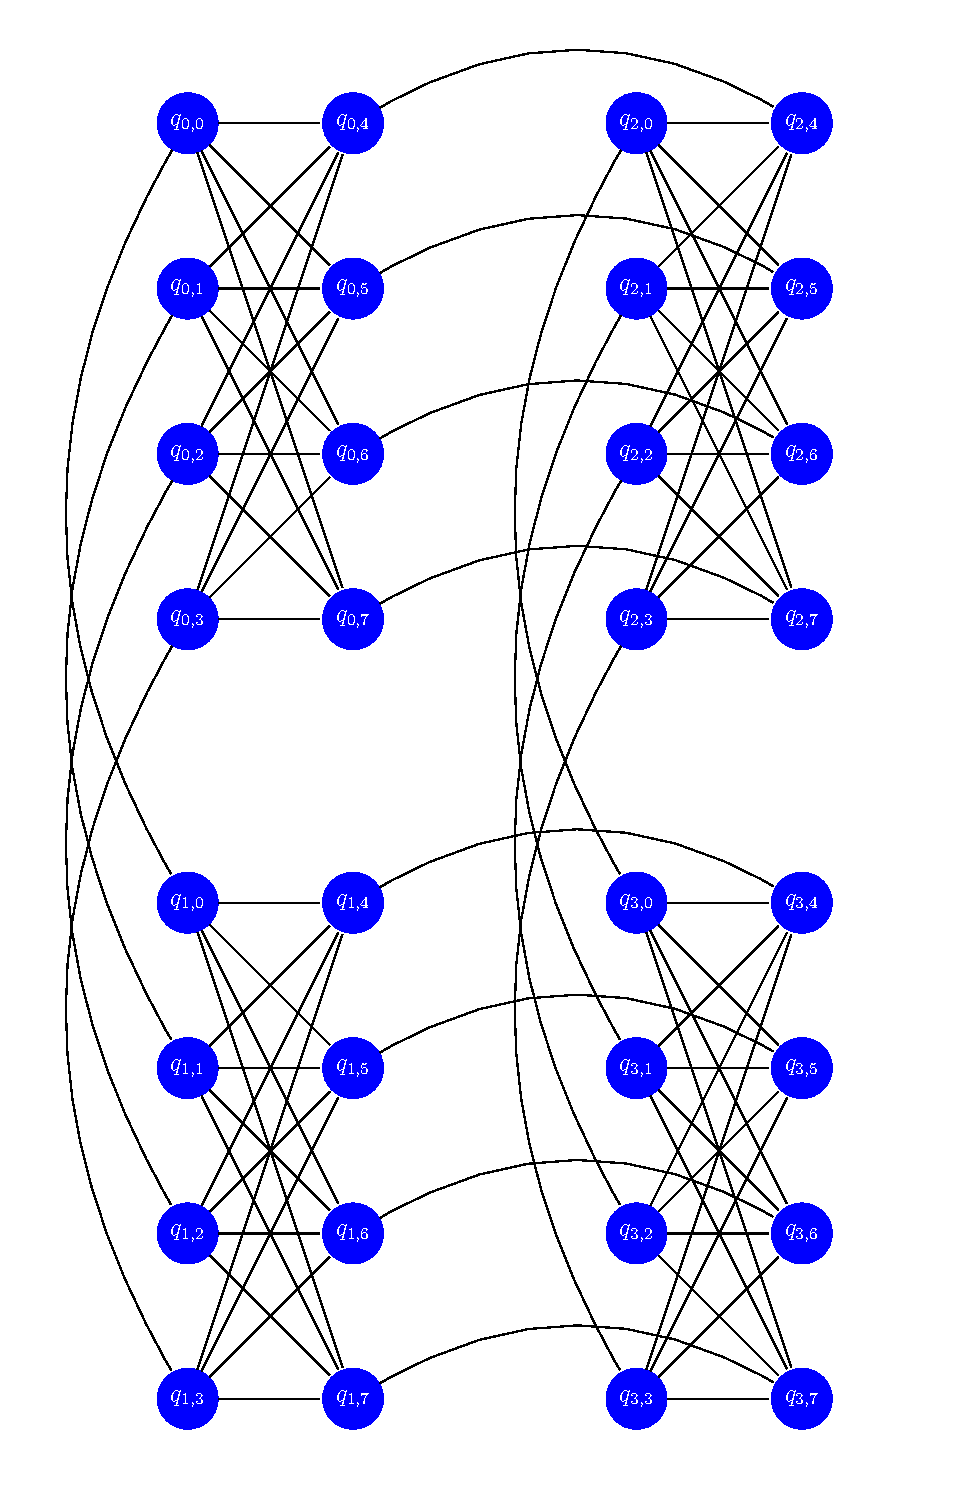
\includegraphics[width=0.45\textwidth]{fig1a.pdf}$\qquad$
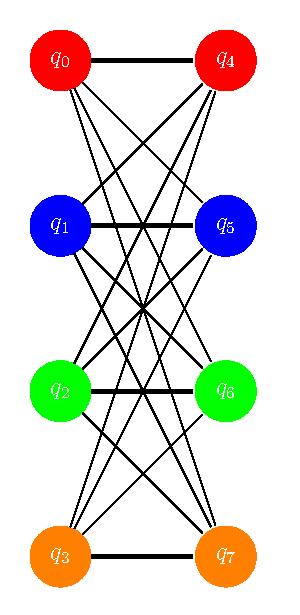
\includegraphics[width=0.35\textwidth]{fig1b.pdf}
\caption{Finding a physical embedding: this figure shows a toy 32 qubit system demonstrating the Chimera graph structure (left) and a synthesized dense network on an individual unit cell (right). The Chimera graph consists of bipartite 8-qubit unit cells as shown, with sparse connections between cells.
To synthesize a dense 4-qubit network on any individual unit cell, negative coupler weights (shown in bold) are added.
I.e., $J_{0,4} = J_{1,5} = J_{2,6} = J_{3,7} < 0$.
}
\label{fig:chains}
\end{figure}

To measure the optimality of an implementation, it is typical to consider both the number of physical qubits $N'$ required to embed the Hamiltonian and the size of the physical energy gap $\Delta'$.
In general, to implement a classical circuit on a QA machine, the circuit must be transformed into a Hamiltonian whose ground states correspond to valid input/output combinations as illustrated in Figure \ref{fig:xor-ex}.
During this process, it is common to introduce ancillary qubits, which are important terms in the Hamiltonian, but do not contain any useful information on input or output.
Using basic gates generated via the above process, it is possible to implement general classical circuits using the additive property of Hamiltonians \cite{pakin2018performing}.
While this methodology is convenient, it is wasteful in terms of ancillary bit requirements, and therefore a hand-crafted solution is preferable for most problems.

\begin{figure}
\centering
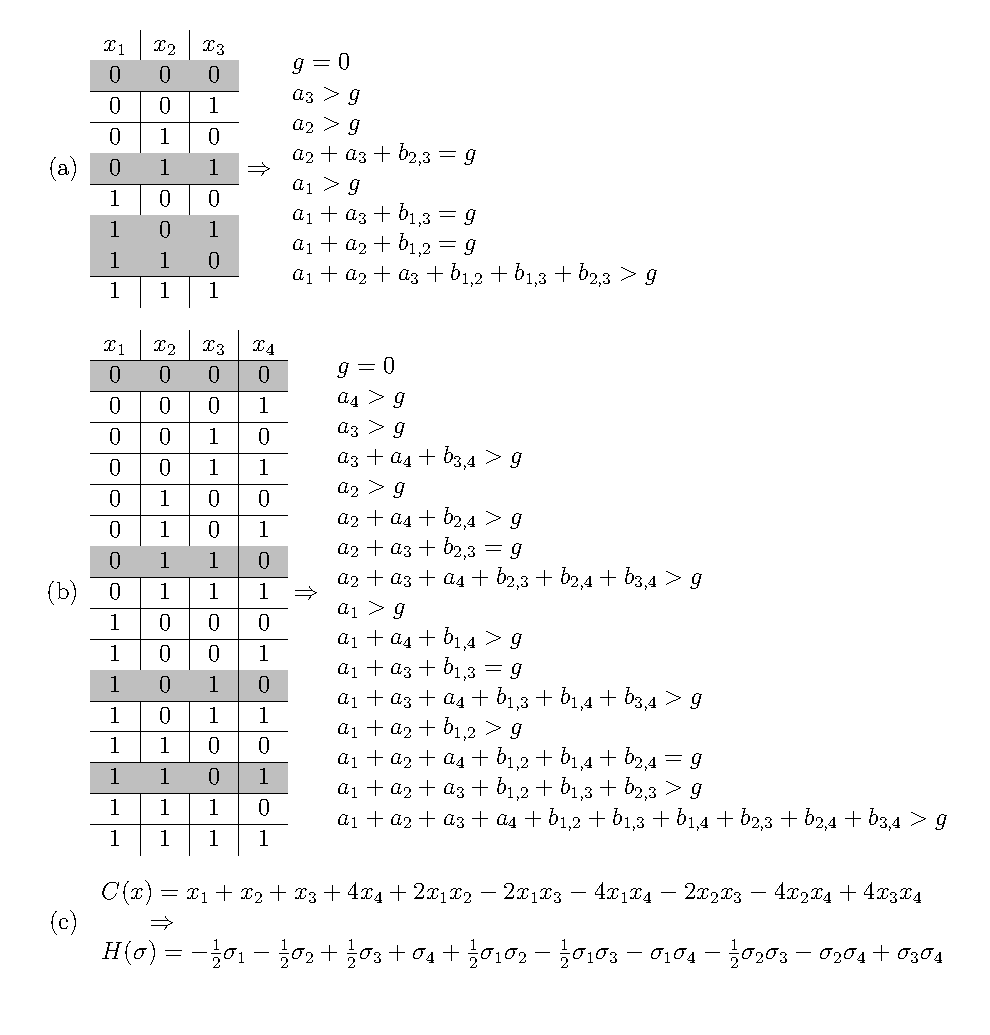
\includegraphics[width=0.9\textwidth]{fig2.pdf}
\caption{Embedding a quantum XOR gate: this figure illustrates the process of programming a quantum annealer, by embedding an XOR gate. The goal is to implement the circuit $x_1 \oplus x_2 = x_3$.
The truth table in (a) shows all combinations of $x_1$, $x_2$, and $x_3$, with all 4 valid input/output combinations highlighted.
Using the QUBO model, this generates the algebraic system of inequalities shown on the right hand side, where $g$ denotes the ground energy of the system.
Because the row containing all zeros is a valid solution, $g$ must be $0$.
The system of inequalities for (a) has no solution, so an ancillary bit $x_4$ is introduced in (b).
There are $2^4$ ways to assign the value of $x_4$ for the $4$ valid states from (a), some of which produce solvable systems and some of which do not.
By trial and error, the rows highlighted in (b) produce a solvable system, shown on the right hand side.
Solving this system produces the QUBO shown in (c), and applying the isomorphism results in the Hamiltonian below.
}
\label{fig:xor-ex}
\end{figure}

Using the transformation $\sigma_i = 2x_i - 1$ and dropping constant terms (which offset the energy landscape, but do not affect the locations of the minima), the Ising model is isomorphic to the quadratic unconstrained binary optimization (QUBO) model
\begin{equation}
C(\mathbf{x}) = \sum_{i=1}^N a_i x_i + \sum_{i=1}^N \sum_{j=i+1}^N b_{i,j} x_i x_j
\label{eq:QUBO}
\end{equation}
where $x_i\in\{0,1\}$ are abstract binary variables, $a_i = 2\left(h_i-\sum_j J_{i,j}\right)$, and $b_{i,j} = 4J_{i,j}$.
For dealing with binary representations of fixed-point numbers, the QUBO model is more convenient and will be favored in Section 3.
However, for performance analyses (Section 4) it is more accurate to consider the Hamiltonian model, which better describes the physical embedding.

The general problem of finding a least squares solution to a system of polynomial equations is equivalent to globally solving a multivariate SOS polynomial minimization problem.
This class of problems should not to be confused with the class of polynomial least squares problems, which refer to the fitting of a polynomial to data by solving a linear least squares problem.
Since SOS problems are known to be NP-hard, classical solutions focus on iterating toward a solution by solving sequences of linear matrix inequality problems \cite{lasserre2001global}.
In the special case where the system of polynomial equations is consistent, the problem can often be efficiently solved using homotopy methods \cite{watson1997algorithm}.
In the special case of linear and least squares systems, these problems can be solved with cubic complexity using standard matrix factorization techniques \cite{golub2012matrix}.

It should be noted that the current generation of D-Wave machines are not capable of solving any meaningfully large SOS problems.
In fact, the elementary operation of multiplication/factorization is considered difficult for these D-Wave machines, due to the practical limitations of D-Wave's technology \cite{andriyash2016boosting}.
Related to some of the applications discussed, a good deal of work has been put into integer factorization, with a focus on security applications.
While Shor's algorithm has become synonymous with quantum factorization, quantum annealing requires a different model \cite{shor1999polynomial}.
Early work in quantum factorization was pioneered by Peng et al., who produced a general model for integer factorization \cite{peng2008quantum}.
Jiang et al.\ expanded on this work in the special case of biprime factorization \cite{jiang2018quantum}.
Dridi et al.\ proposed an alternative approach to biprime factorization using Gr\"{o}bner bases \cite{dridi2017prime}.
In general, to factor an $n$-bit binary integer, these approaches require $\mathcal{O}(n^2)$ qubits and result in an exponentially decaying physical energy gap $\Delta'$.
It is also worth mentioning a hybrid quantum-classical algorithm for nonlinear integer programming, proposed by Alghassi et al.\ \cite{alghassi2019graver}.

For the special case of solving systems of linear equations, quantum algorithms have been proposed for both the gate model \cite{PhysRevLett.103.150502} and AQC model \cite{PhysRevLett.122.060504,PhysRevA.99.012320} that achieve exponential speedup in cases where the associated matrix has a low condition number.
For QA, there are two closely related works that were recently published, both of which achieve a QA solution by embedding the error function in the Ising-Hamiltonian.
Borle et al. \cite{borle2019analyzing} propose this methodology for solving linear systems of equations and least squares problems, but refrain from analyzing higher-order systems.
Chang et al. \cite{chang2019quantum} propose this method for finding least squares solutions to general systems of polynomial equations, but use a slightly different binary encoding technique, where fixed-precision signed arithmetic is achieved via a linear transformation of unsigned binary integers. The present work accompanies \cite{borle2019analyzing,chang2019quantum} by providing both an extension to higher order systems and an easily accessible coding framework for solving arbitrary polynomial SOS problems on a QA system.